\section{Methods}
\lb{sec:methods}

Our methodology for classification was dependent on two things: The data that we had, which needed to be cleaned and the algorithms that we needed to apply. For this we decided on using the 3rd catalog of F-LAT (3FGL from hereon) for initial training and testing, the 4th catalog (FL8Y from hereon) for further testing and predictions, and machine learning algorithms like Random Forests, Logistic Regression, Decision Trees, and Neural Networks. All of the machine learning algorithms were taken from the python module sklearn, including Neural Networks. A neural network using Keras was also attempted; however, due to the classification being on only two classes, we discarded it in favour of the sklearn algorithm which was much faster.\\

Our data was similar to that used by Parkinson et. al. We cleaned the 3FGL catalog to have sources which were both associated and unassociated but with no missing values. We then used the associated sources which were classified as either AGNs (with multiplpe labels) or Pulsars, to get a list of 1905 sources. The rest of the sources without problematic values were then used as unassociated sources, which we used later on for testing and prediction. The FL8Y presented us with another way of testing the accuracy of our methods. We predicted the classifications of unasssociated sources in the 3FGL and used the FL8Y to check how many of these unassociated sources, which now had associations in the FL8Y, actually had the right prediction.\\

The raw data of the catalog had a lot of different features that could be used for classification. However, going by the previous studies, we decided on using the most important features, which included Flux density and the error on it, spectral index, the curvature, hardness ratios (as defined by Parkinson et. al.), variablity, and also the galactic latitude, the last of which was used even in the classification of AGN and Pulsars (as opposed to Parkinson, who used it only for the young and milli-second pulsar distinction). In features where the values were high, we used the logarithmic scale to better seperate the sources. The complete list of sources, along with some statistics, is given in the table below. The influence of the features on the classification, especially the differences in the various methodologies is discussed in much more detail in the next section.\\

One of the main aims of our project was to understand and optimize the machine learning methods which we were using. So apart from the features which were in the data itself, we also theorized and experimented with the parameters of the algorithms themselves. We wanted to find the fastest and cost-effective way of using certain methods, without going into regimes of under and over-fitting the data. Parameters which we studied range from Depth and Number of trees in Forest based methods to the number of hidden layers and epochs in neural networks. The details are given in the next section, where we discuss our expectations and the resulting behaviour of our algorithms.\\
  
In our general the Methodology was as follows.
\ben
\item
Split the PS with known classification into learning and test samples.
\item
Use the learning sample for training and for selection of features.
In particular, continuous parameters, such as the thresholds in the decision trees or mixing matrices in neural networks, are determined from the learning sample. 
\item
Meta-parameters, which encode the complexity of the methods, such as the depth of the decision trees,
are determined from the best performance on the test sample.
\een

After the above had been completed we were ready both with our final data and our optimum algorithms. We then applied and sought the results using both the catalogs in our possession. This is discussed in detail in section 4 and 5.\\


When applied on the 3FGL known sources, using 1500 sources to train and the rest to test on, we found (for 10 seeds) the following: \\

\begin{table}[!h]
    \tiny
    \centering
    \renewcommand{\tabcolsep}{1mm}
\renewcommand{\arraystretch}{1.5}

    \begin{tabular}{|c|c|c|}
    \hline
    Algorithm Name&Parameters & Accuracy\\
    \hline
    Random Forest& 50 trees and 12 max depth & 97.91        \\
    \hline
    Neural Network & 200 epochs and 20 neurons in 1 layers       &  98.2 \\
    \hline %\midrule   -> aakash do you mean this?
    Gradient Boost& 50,15      &   96.78  \\
    \hline %\midrule   -> aakash do you mean this?
    Logistic Regression& all solvers &<94  \\
    \hline
     
    \end{tabular}

    \caption{Testing Accuracy of 4 algorithms on 3FGL data}
    \label{tab:my_labe2l}
\end{table}

\subsection{Details of the analysis}

\subsection{Data and Features}

The total number of sources, including unassociated and associated, in the two catalogs is shown below. \\
\begin{figure}[h]
%\centering
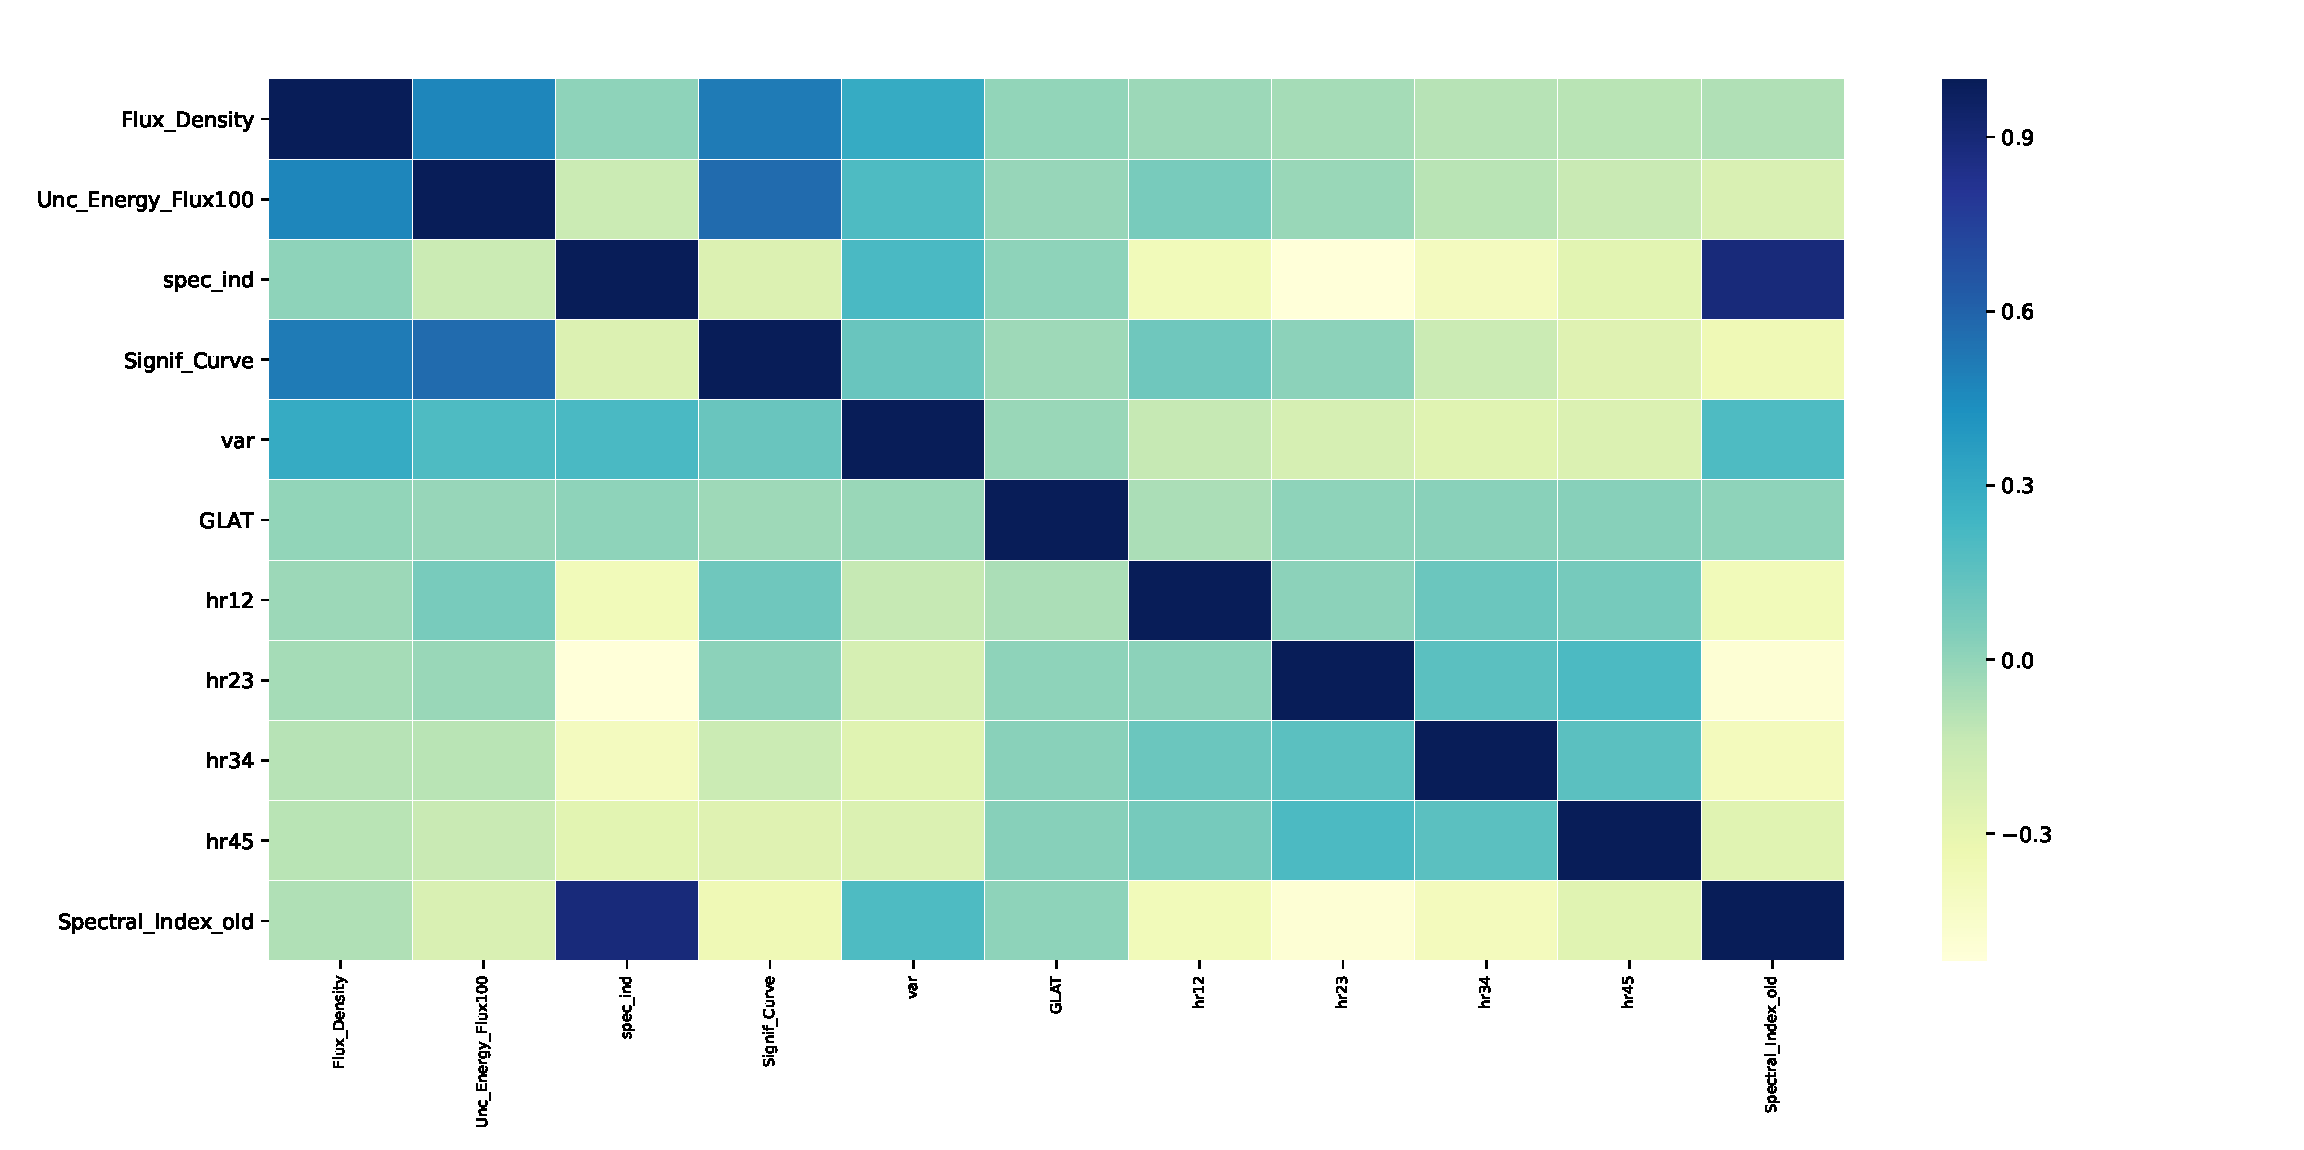
\includegraphics[width=\onepic\textwidth]{plots/correlation.pdf}
\caption{Correlation matrix for the most important features}
\label{fig:corr}
\end{figure}
[Add Table]\\

The features used for our analysis follow the same idea as the previous studies. The features, along with statistical and methodological details, are given below. A correlation matrix is presented for the most important features as well. The matrix is important for the case where there might be redundant features, in which case using only one of the two features would be a better idea.\\



[Add Table of features for both catalogs]\\

Our initial hypothesis was that certain features would be more important for classification than others. For instance, as shown below, one can see a clear distinction between the regimes of AGNs and Pulsars, based on spectral idex and significant curvature. [Add image] While not clearly obvious from the get go, we were also interested in comparing the importance of features based on the algorithms that we were using. Due to the difference in the basic method of Random Forests and Neural Networks, we expected a slight shift in their reliance on certain features. Despite that we hypothesized that features with the most contribution would be among spectral index, variability, and the curvature; as already observed by Parkinson et. al.\\

\begin{figure}[h]
%\centering
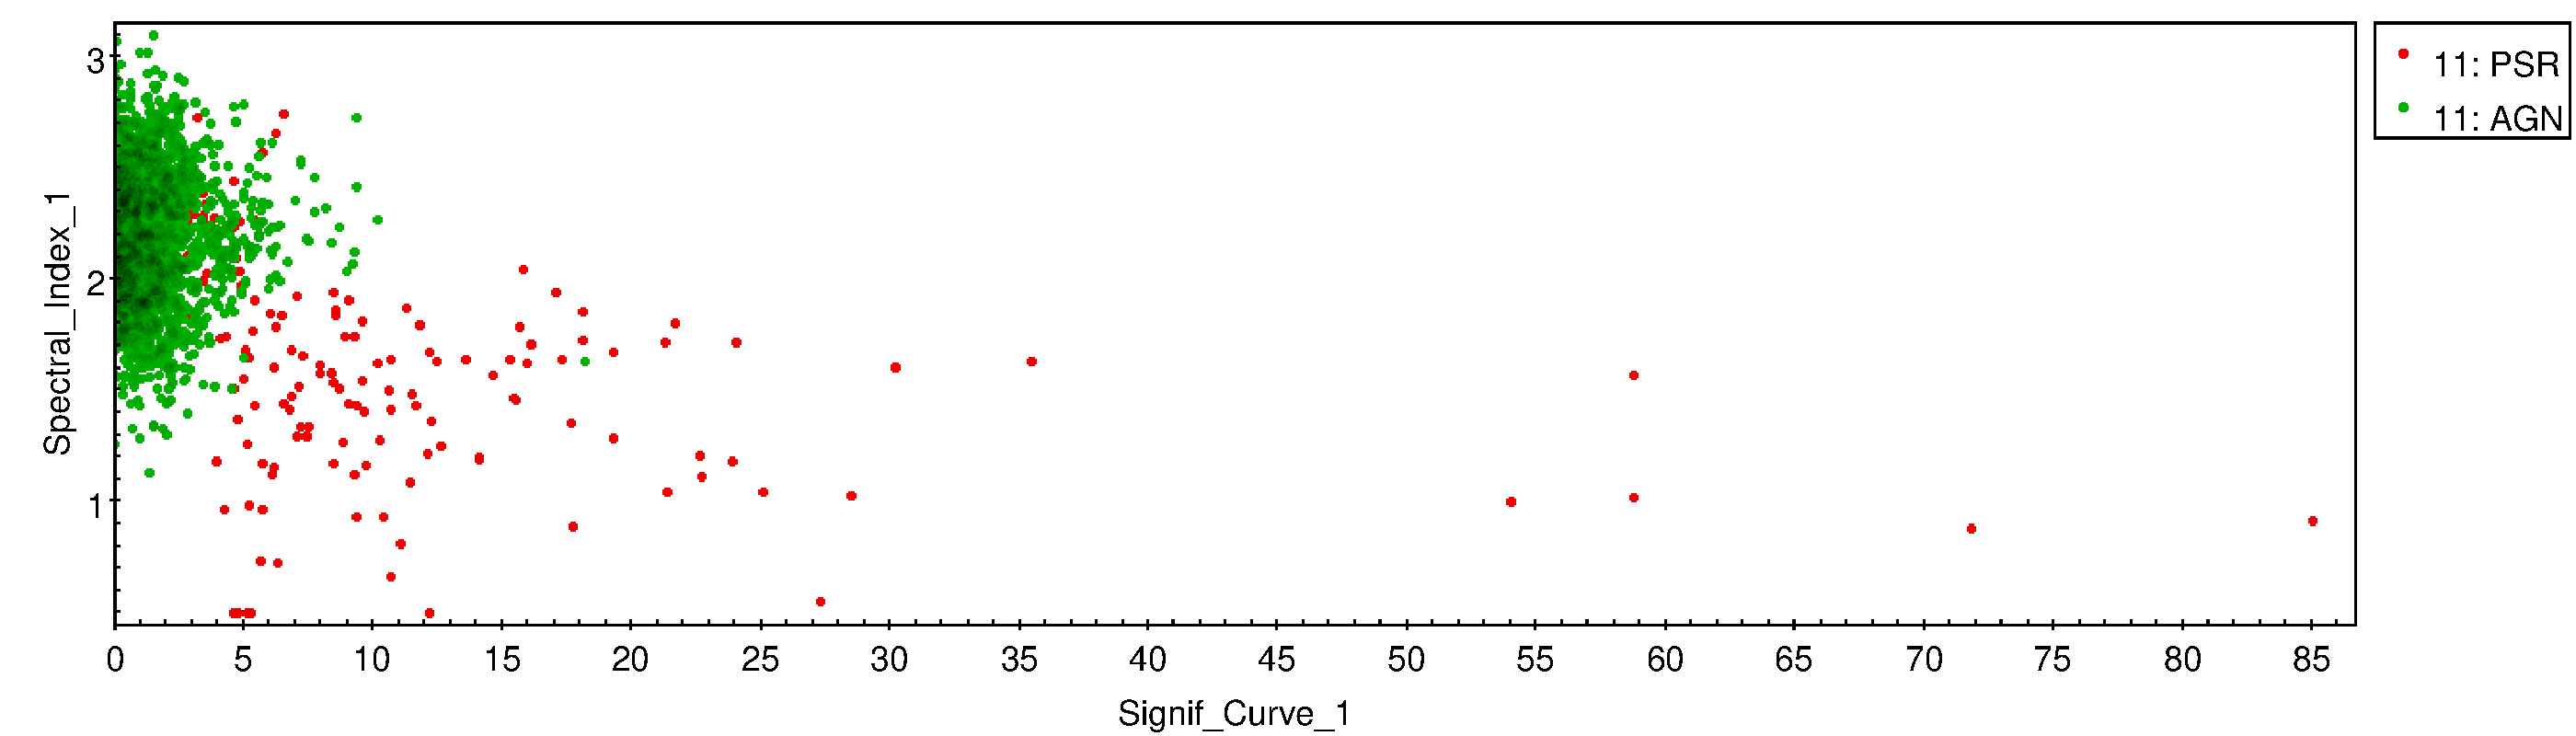
\includegraphics[width=\onepic\textwidth]{plots/signifcurvvsspecind.pdf}
\caption{Differences in AGNs and PSRs from the 3FGL catalog}
\label{fig:corr}
\end{figure}


\subsection{}


\ben
\item
Describe the features that we use for the analysis.
\item
Describe the objective function for minimization (accuracy of classification on learning sample).
Weighted objective function: give more weight to pulsars, since there are fewer of them in the catalog.
\item
Learning curve using all features?
{\it Plot: classification accuracy using the total list of features for learning and test sample as a function of complexity parameter.}
\item
Selection of the most important features.
{\it Table: features vs algorithms. Columns: algorithms, rows: features, values: significance.}
\item
Selection of meta-parameters.
{\it Plot: classification results for the test sample using a subset of features.}
\item
Train the final classifier.
{\it Table: classification accuracy of the final classifiers for different algorithms using the test sample from 3FGL.}
\een

Discuss the general features of the optimal algorithms: which features turn out to be important, what is the depth of the trees, the number of trees in random forests, the depth and number of internal nodes in the neural networks. \\

\begin{figure}[h]
%\centering
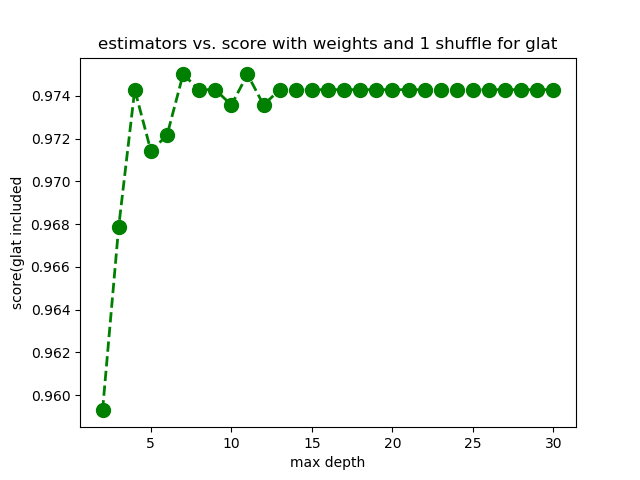
\includegraphics[width=\onepic\textwidth]{plots/Rf_maxdepth_oobscore_glat}
\caption{
Example of a figure for one column.
}
\label{fig:Maps_data}
\end{figure}


\begin{figure*}[h]
%\centering
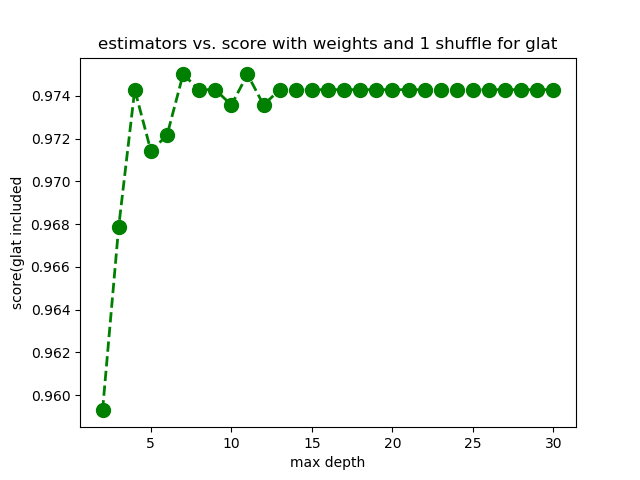
\includegraphics[width=\twopicsp\textwidth]{plots/Rf_maxdepth_oobscore_glat}
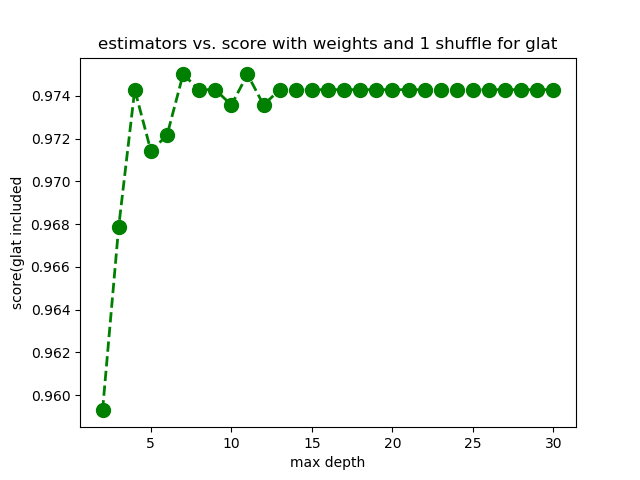
\includegraphics[width=\twopicsp\textwidth]{plots/Rf_maxdepth_oobscore_glat}
\caption{
Example of a figure for both columns.
}
\label{fig:Maps_data}
\end{figure*}

Our hypothesis about feature importances turned out to be correct, as curvature, variability, and spectral index were the most important features. The last hardness ratio was also seen to be quite important, most probably reflecting the end of the spectrum where the AGNs and PSRs shift from each other. These values are given in the table below. \\

\begin{table}[!h]
    \tiny
    \centering
    \renewcommand{\tabcolsep}{1mm}
\renewcommand{\arraystretch}{1}

    \begin{tabular}{|c|c|c|}
    \hline
    Feature Name&  RF (50,15)& GB (50,15)\\
    \hline
    Flux Density& 0 & 0        \\
    \hline
    Unc Energy Flux100& 0     & 0 \\
    \hline %\midrule   -> aakash do you mean this?
   Spectral Index & 0.16      &   0.07  \\
    \hline %\midrule   -> aakash do you mean this?
    Significant curvature& 0.28 &0.47  \\
    \hline
   var&  0.11    &  0.21  \\
    \hline %\midrule   -> aakash do you mean this?
    hr12& 0.06 &0.04 \\
    \hline
     hr23& 0.04 &0.02 \\
    \hline
    hr34& 0.06 &0.04 \\
    \hline
   hr45& 0.22 &0.10 \\
    \hline
    GLAT&0.04&0.01\\
    \hline
    \end{tabular}

    \caption{Feature importances for different Algorithm}
    \label{tab:feat_imp}
\end{table}

These importances were found to be consistent for various different algorithm parameters. So while the value might change a bit for different tree architechtures, for instance, the importances of these features were still pronounced. \\
\subsection{Comparison of the classification algorithms}

{\it Plot: classification domains for a pair of features (or different pairs of features, e.g., latitude vs index, index vs curvature, latitude vs variability).}

Probabilistic classification? Result: probability for a source to belong to a particular class.
Result of classification: table of sources with probabilities for different algorithms.
Final probability: the probability for one of the algorithms (for the most precise one?) and uncertainties determined from the other algorithms.

Discuss a few examples where algorithms give different predictions (are these sources at the boundaries of the domains).

Discuss examples where algorithms misclassify sources from the test sample.\\


In the case of test data, we worked with three different classification algortithms, namely Random Forests, Ada Boost, and Neural Networks. Here we were mostly concerned with tweaking the parameters of the classification algorithms involved, minimizing the cost of computation and aiming for the most efficient way of classification. \\

\subsubsection{Random Forests}


\begin{figure}[h]
%\centering
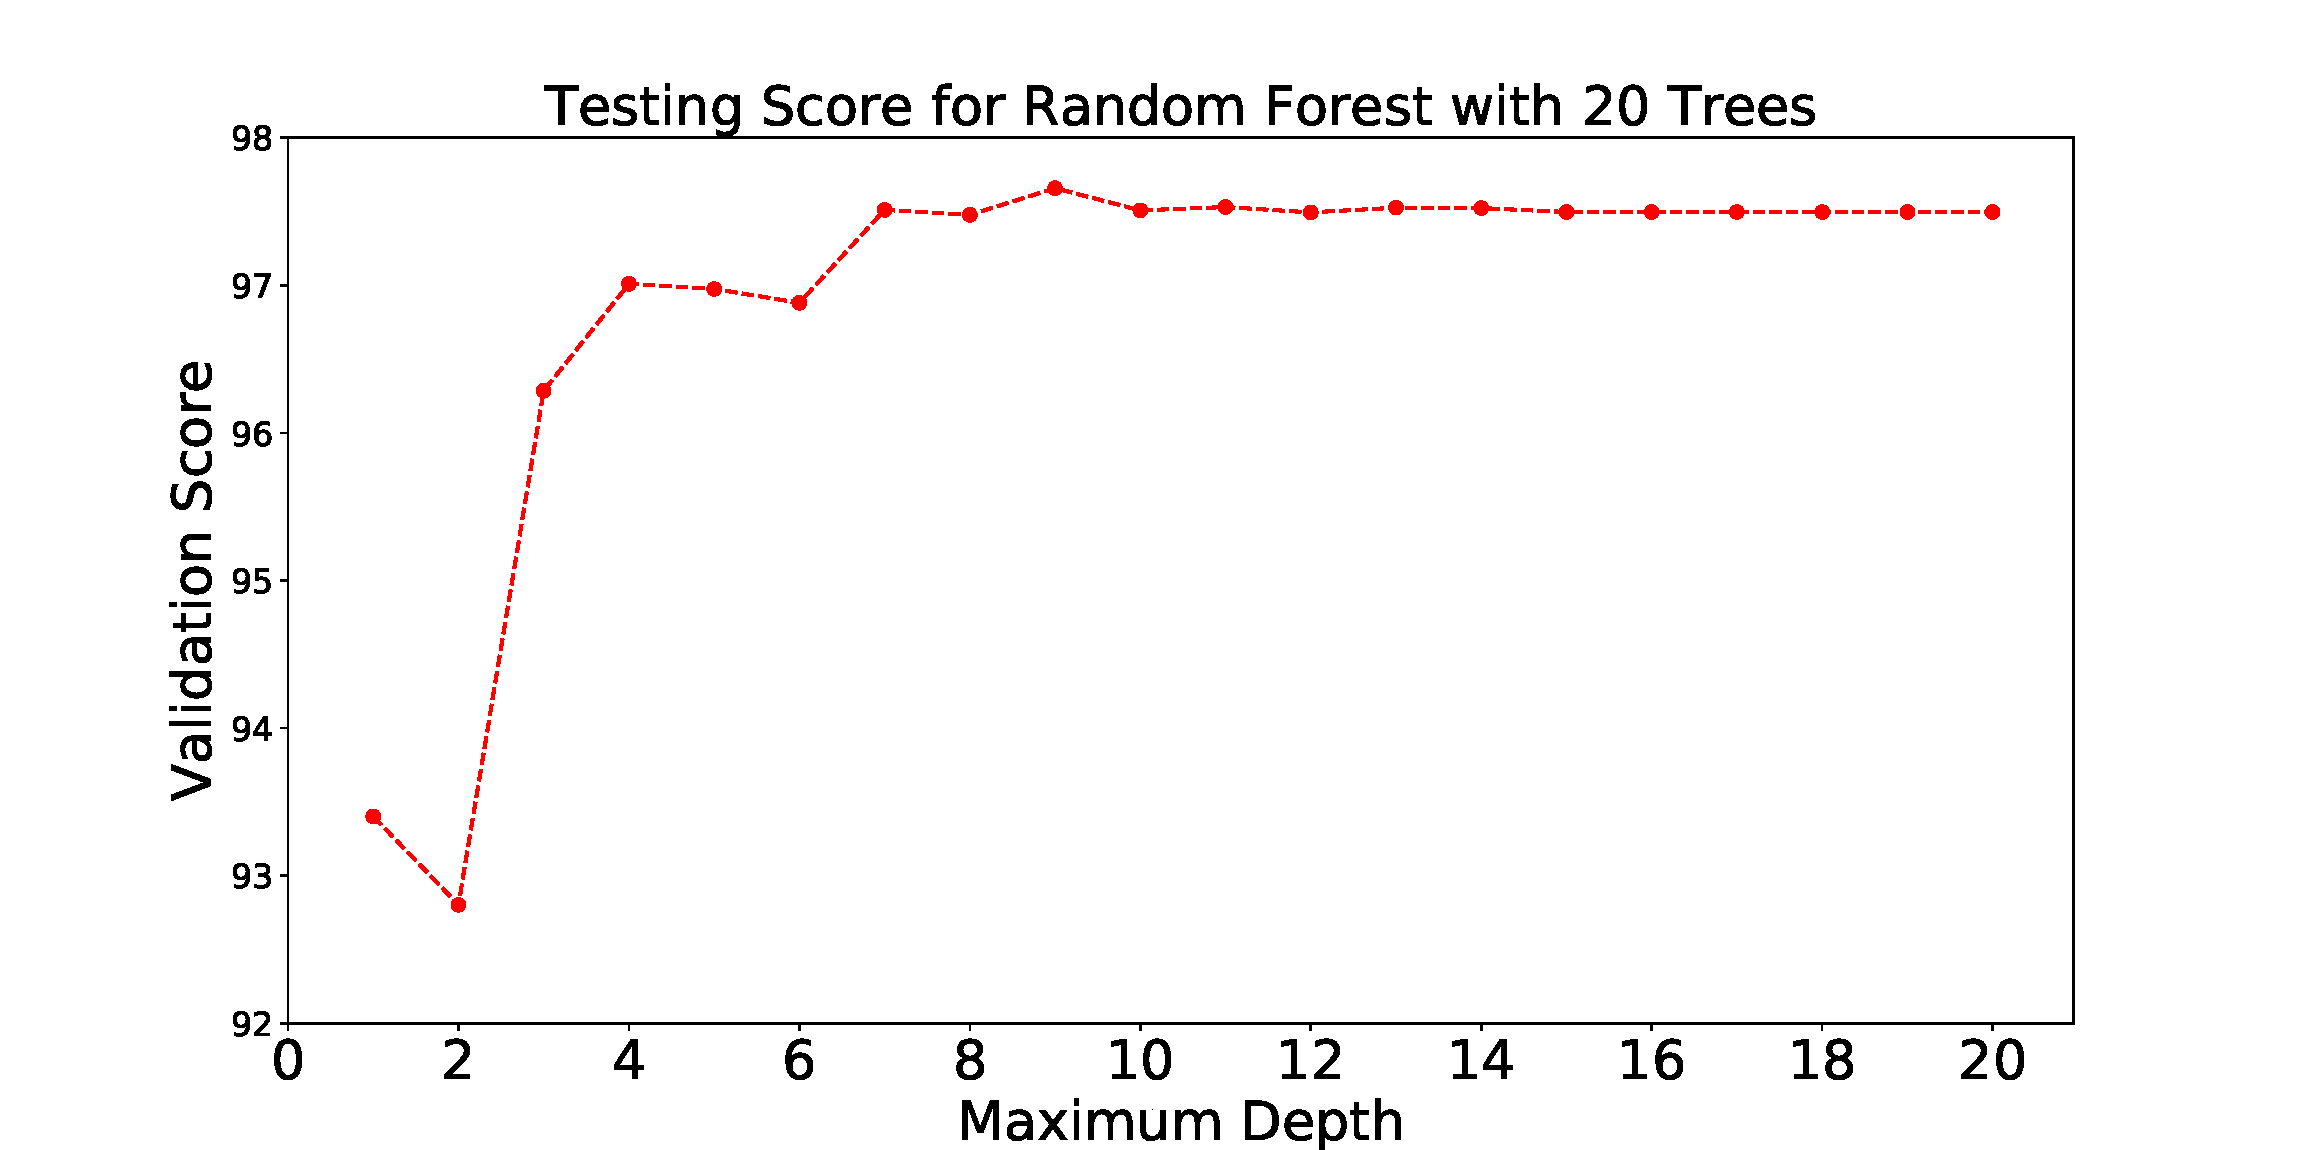
\includegraphics[width=\twopicsp\textwidth]{plots/depthvsscore_rf_10seeds_20trees.pdf} \\
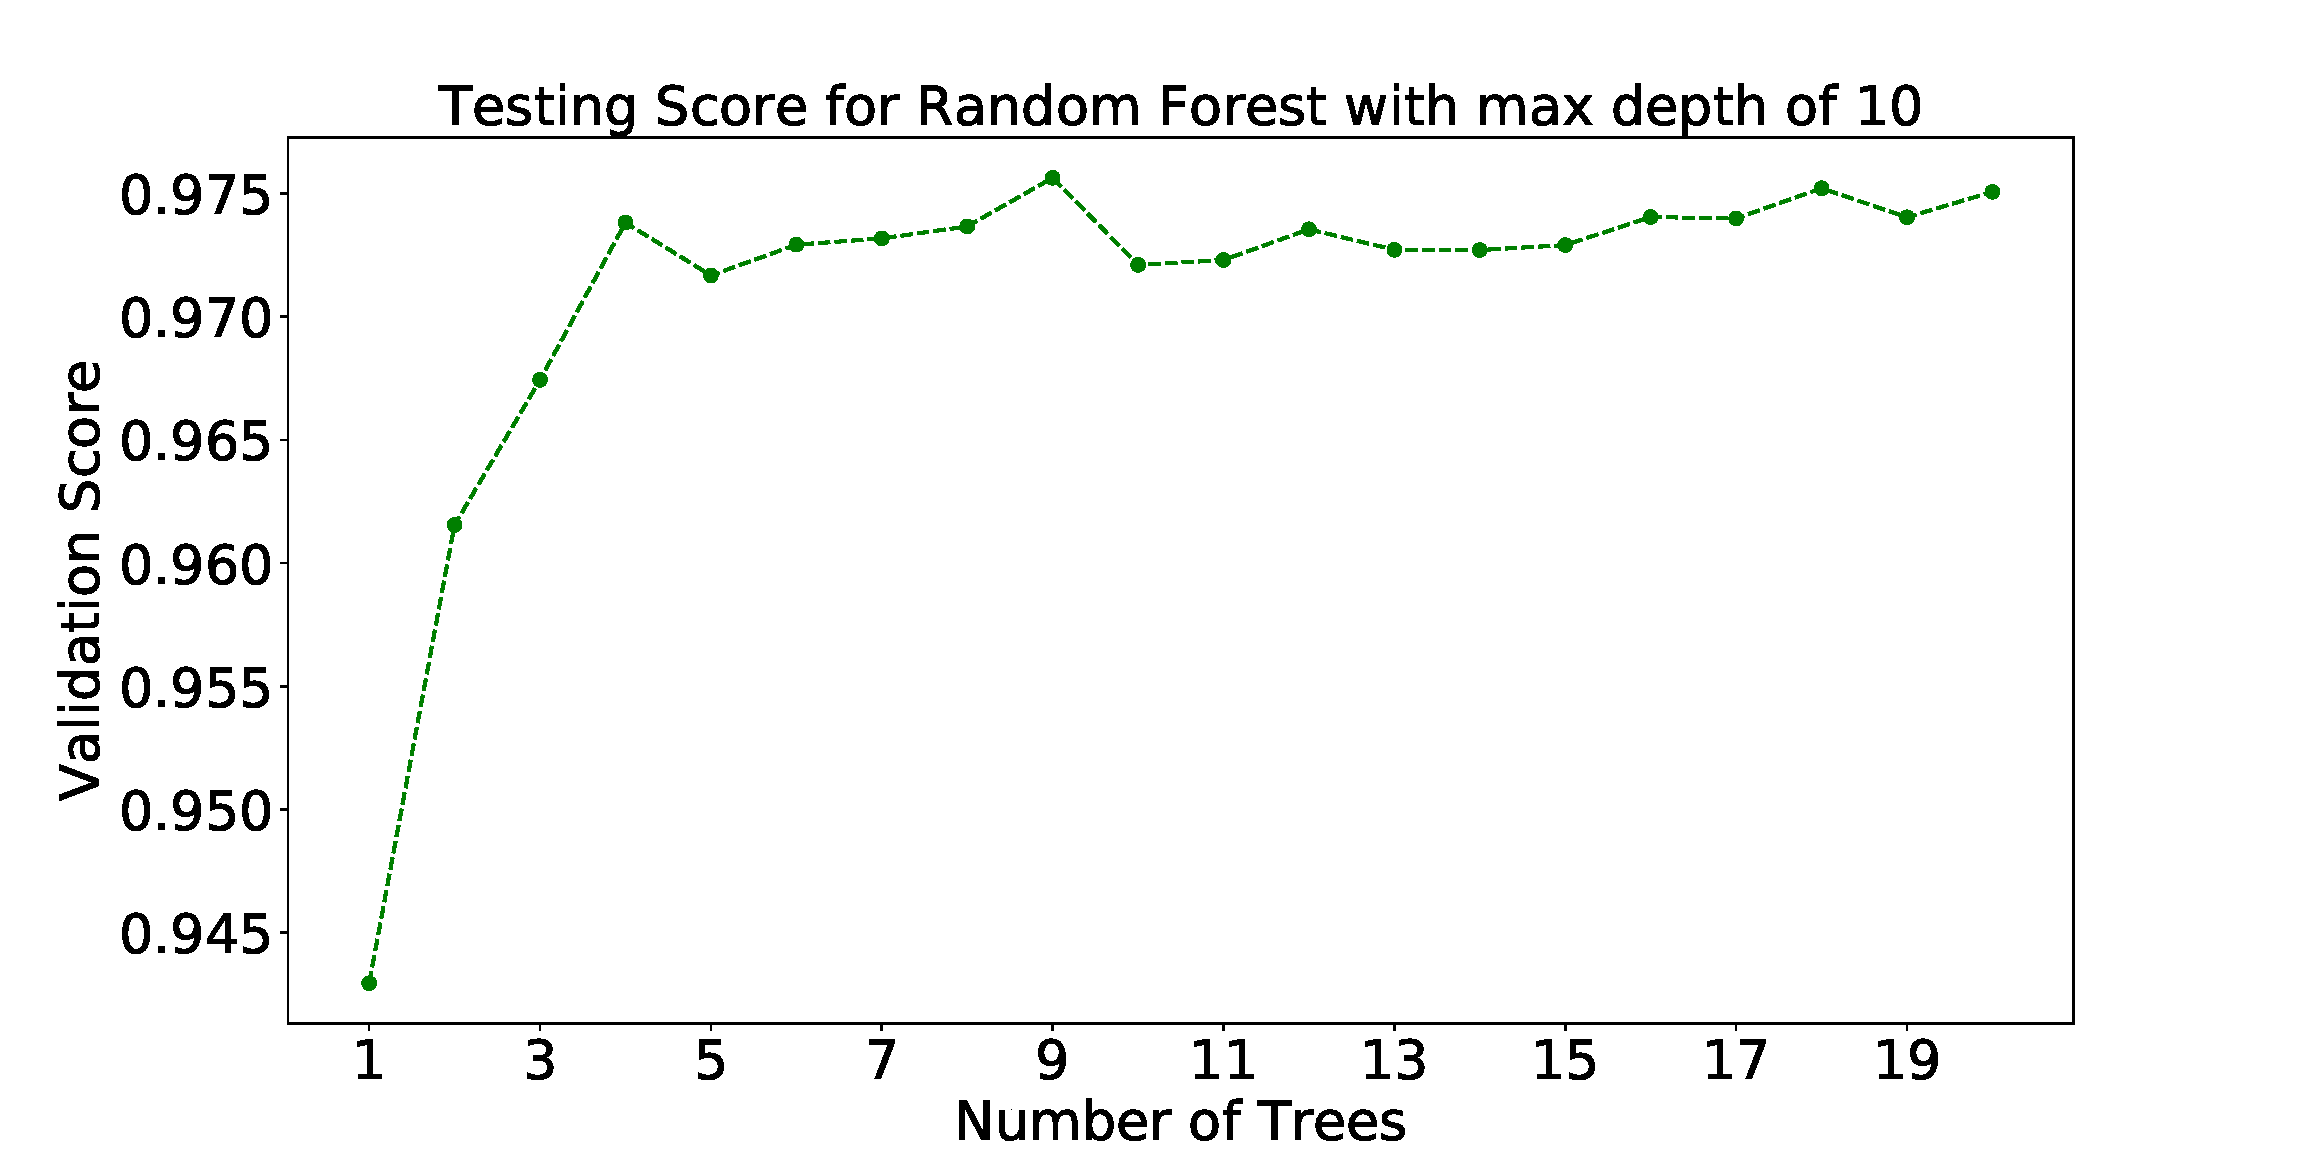
\includegraphics[width=\twopicsp\textwidth]{plots/treesvsscore_RF_10seeds_10maxdepth}
\caption{
Random Forests on Testing Data
}
\label{fig:Maps_data}
\end{figure}

The two main parameters involved in Random Forests are the number of trees and the maximum depth of the trees involved. Figures below shows one instance of the accuracy as a function of maximum depth when the number of trees was kept constant, and as a function of number of trees when the maximum depth was kept constant. \\


\subsubsection{Neural Networks}

In the case of neural networks we were concerned with the number of epochs that one would need to tweak, along with a dependence on the number of neurons in the hidden layers. A final improvement involved checking whether multiple hidden layers would actually add to such a classification algorithm or not.\\
As can be seen in the figure, a complex network with two hidden layers (100 and 5 neurons) reaches the maximum accuracy pretty fast. The results becoming more consistent at higher epochs. A similar result was found for a network having two hidden layers but with only 20 neurons in the first layer. However, such networks could also lead to overtraining, and therefore it is important to check whether such a high accuracy could perhaps be reached by less complicated algorithms, which would drastically reduce the chances of overtraining and allow for a more flexible classificaition methodology.\\

\begin{figure}[h]
%\centering
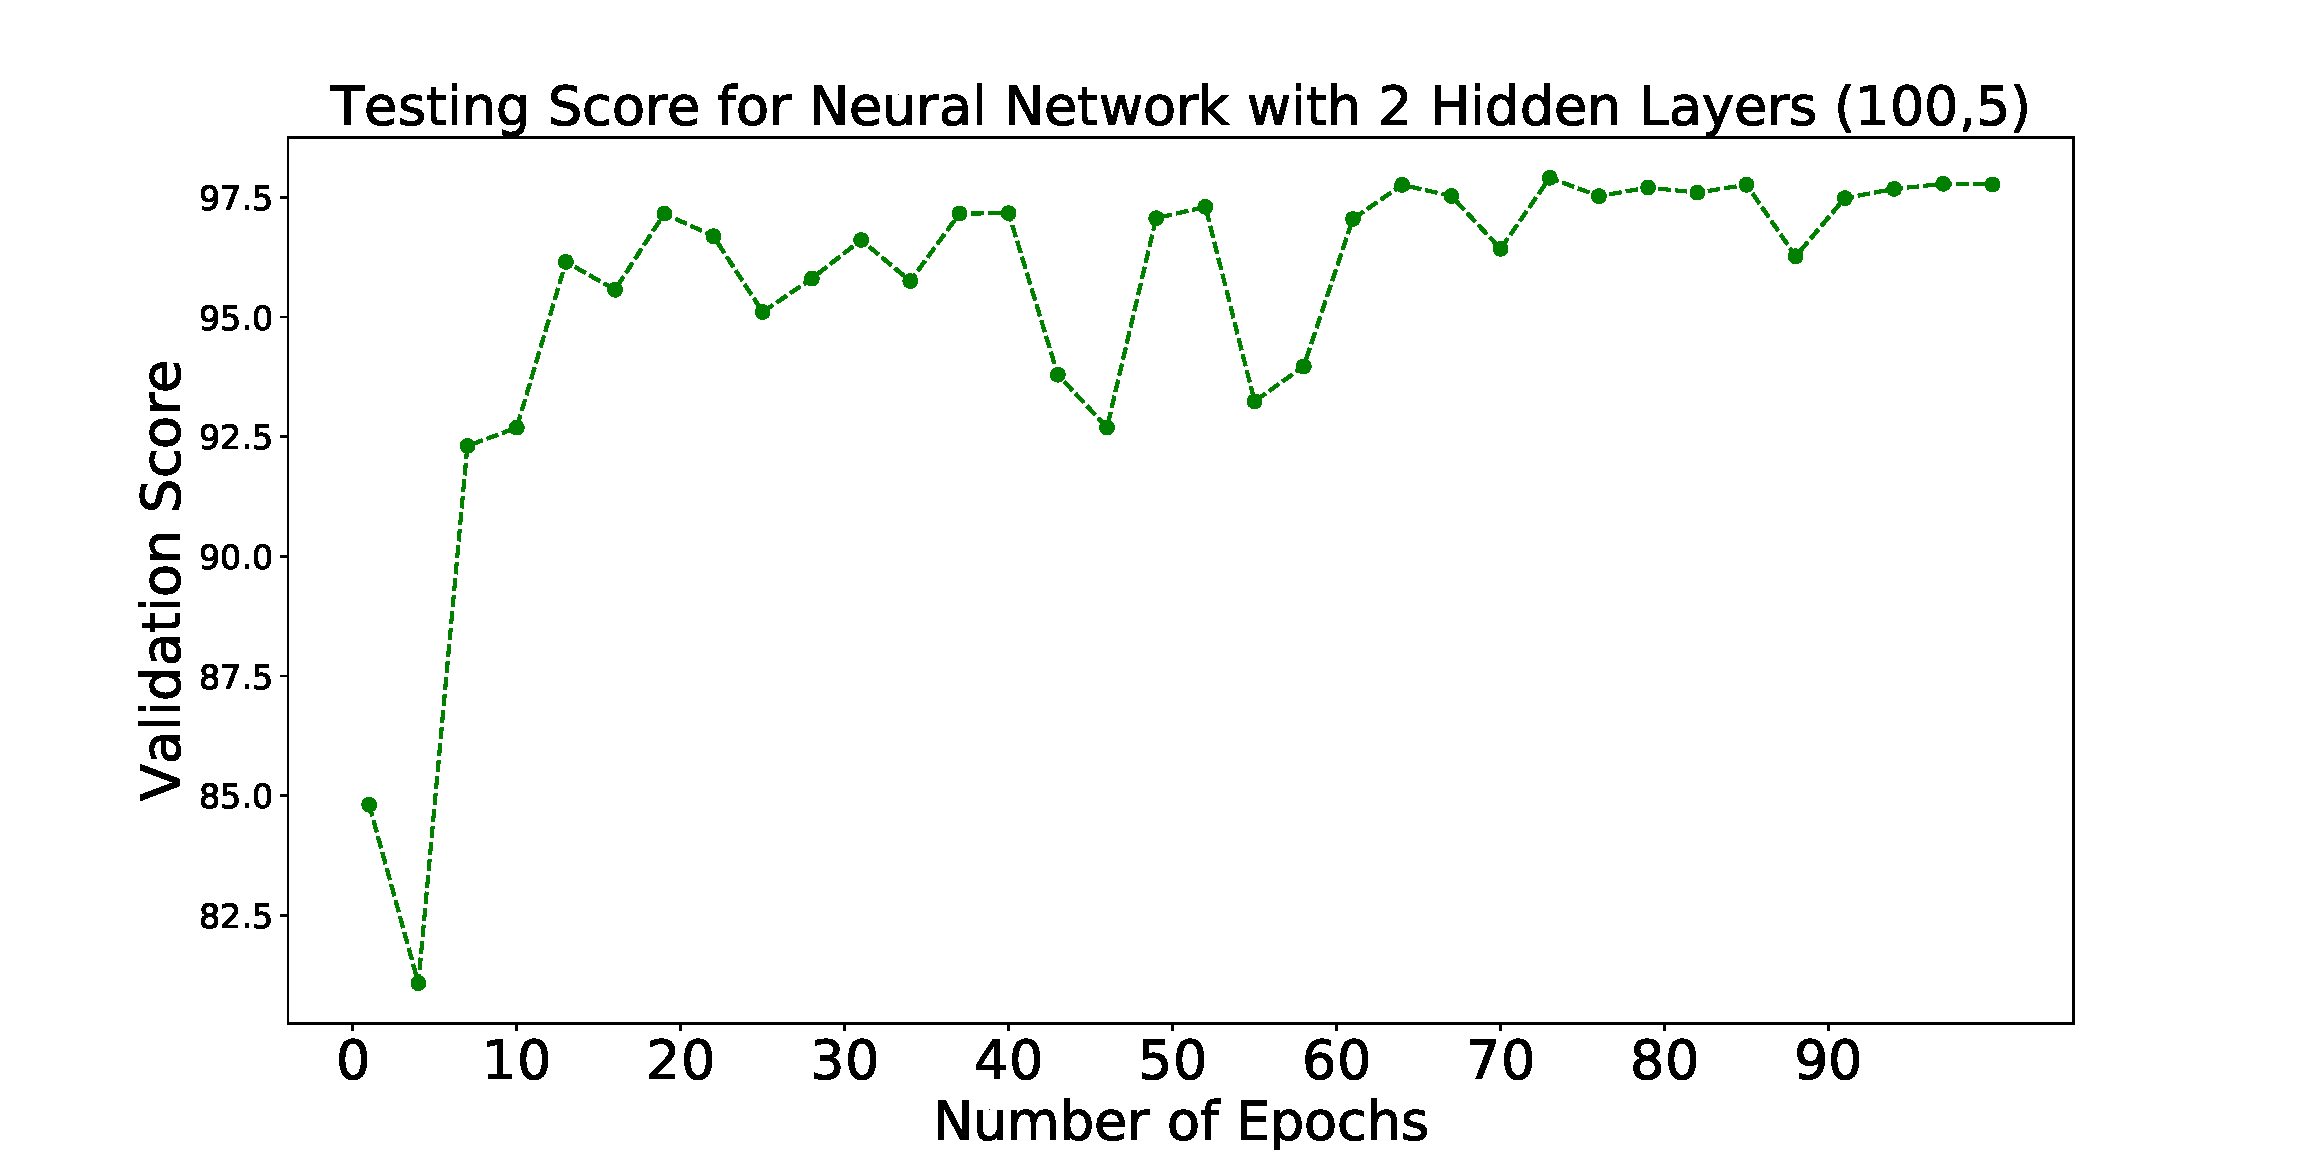
\includegraphics[width=\onepic\textwidth]{plots/epochsvsscore_10seeds_100_2}
\caption{
Example of a figure for one column.
}
\label{fig:Maps_data}
\end{figure}

\begin{figure}[h]
%\centering
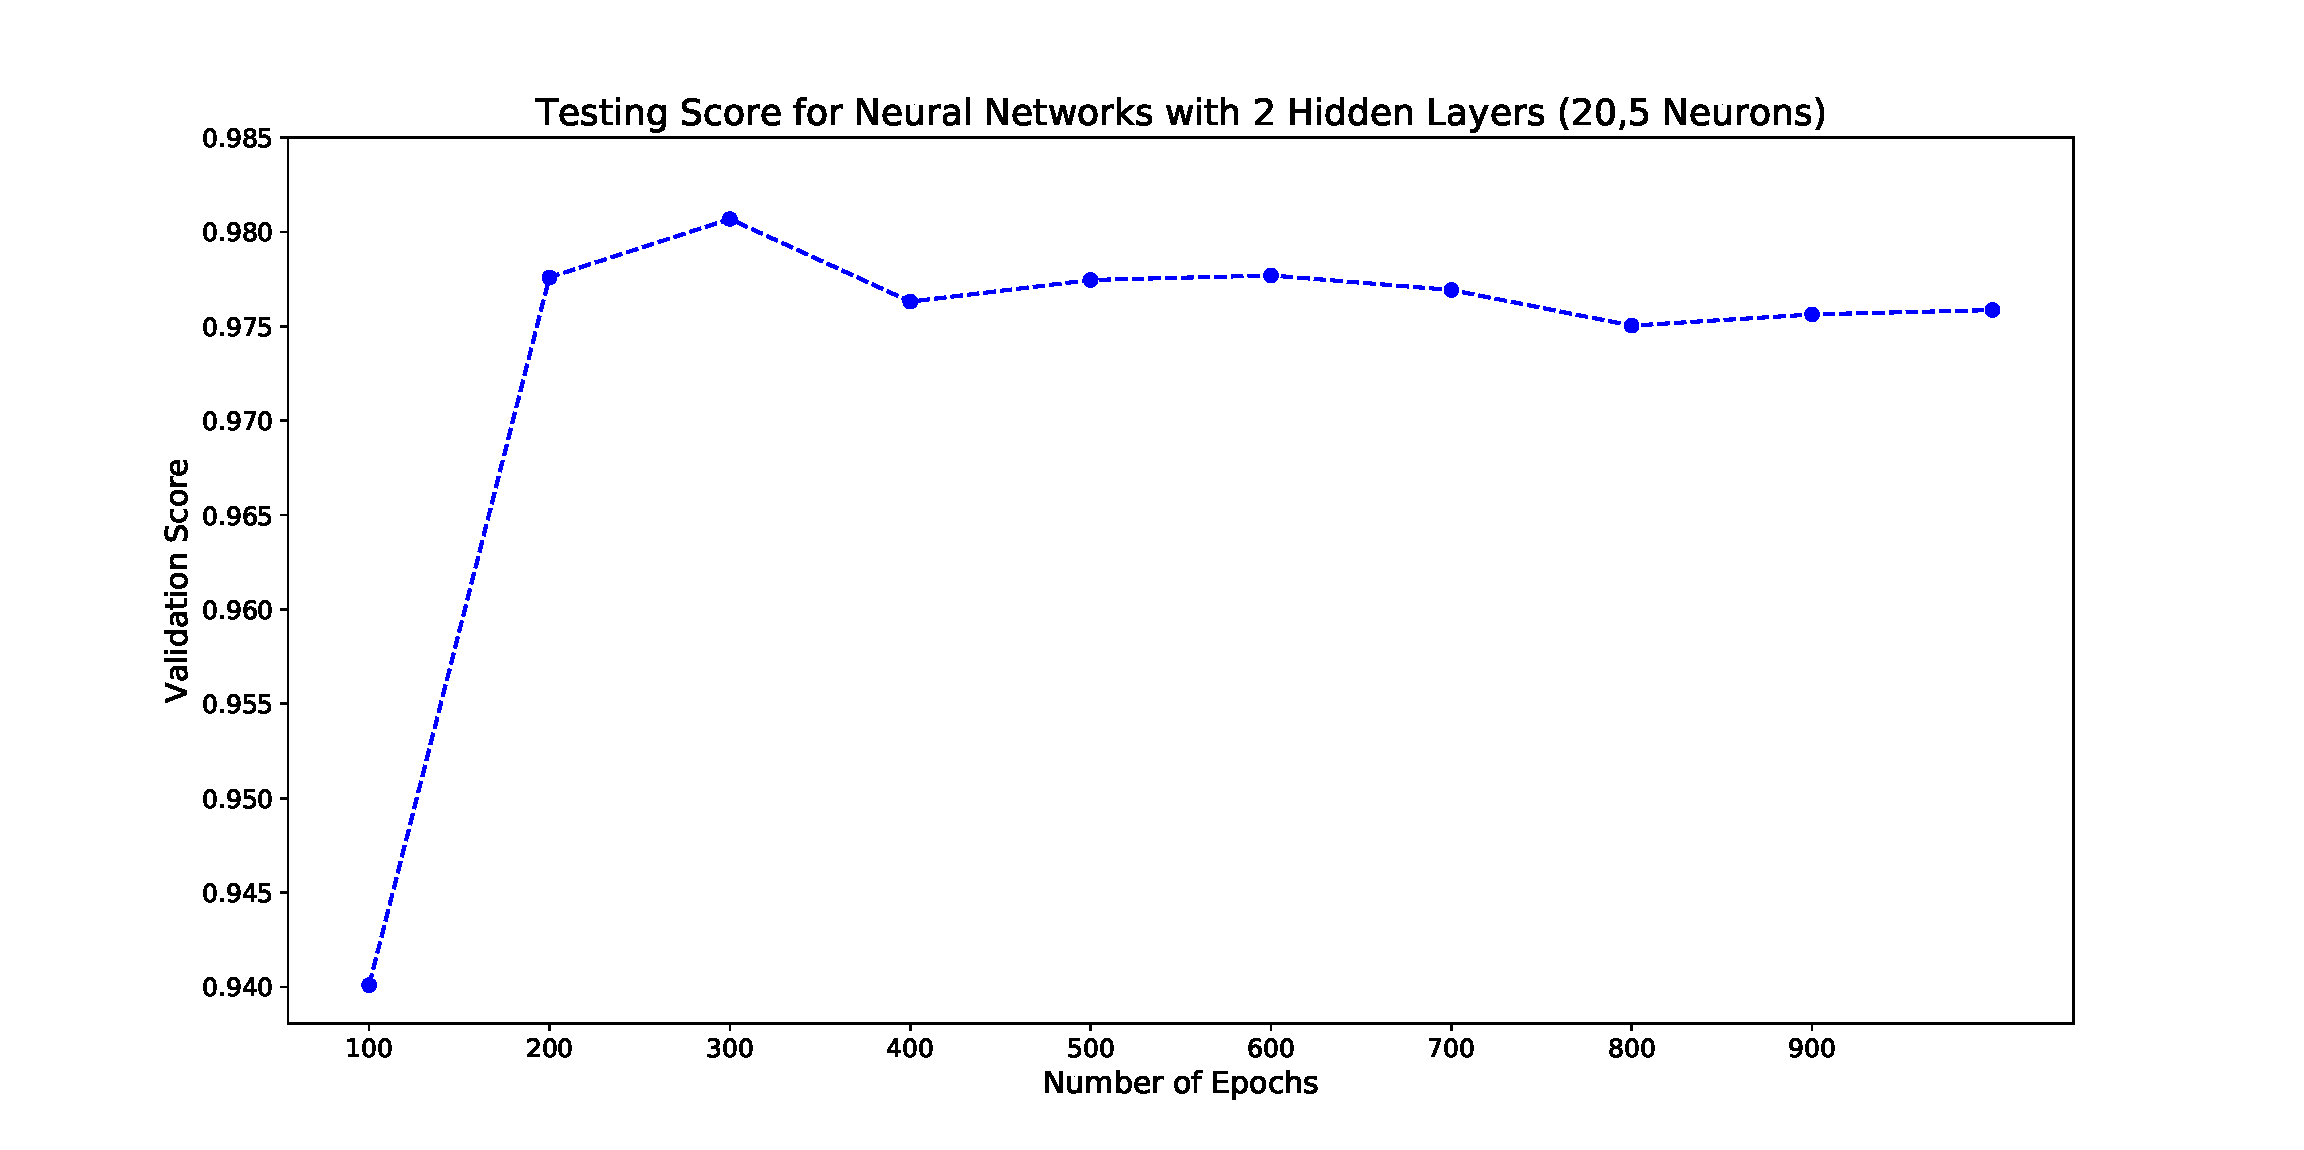
\includegraphics[width=\onepic\textwidth]{plots/epochsvsscore3_10seeds.pdf}
\caption{
Neural Network
}
\label{fig:Maps_data}
\end{figure}

A consistent and accurate result is found even for networks with only one hidden layer with 20 and 5 neurons in the hidden layer respectively. There seems to be no significant dependence for the number of epochs above 30, and even a simple network with one layer and 5 neurons shows a high accuracy for only 30-40 epochs.\\


\begin{figure*}[h]
%\centerin
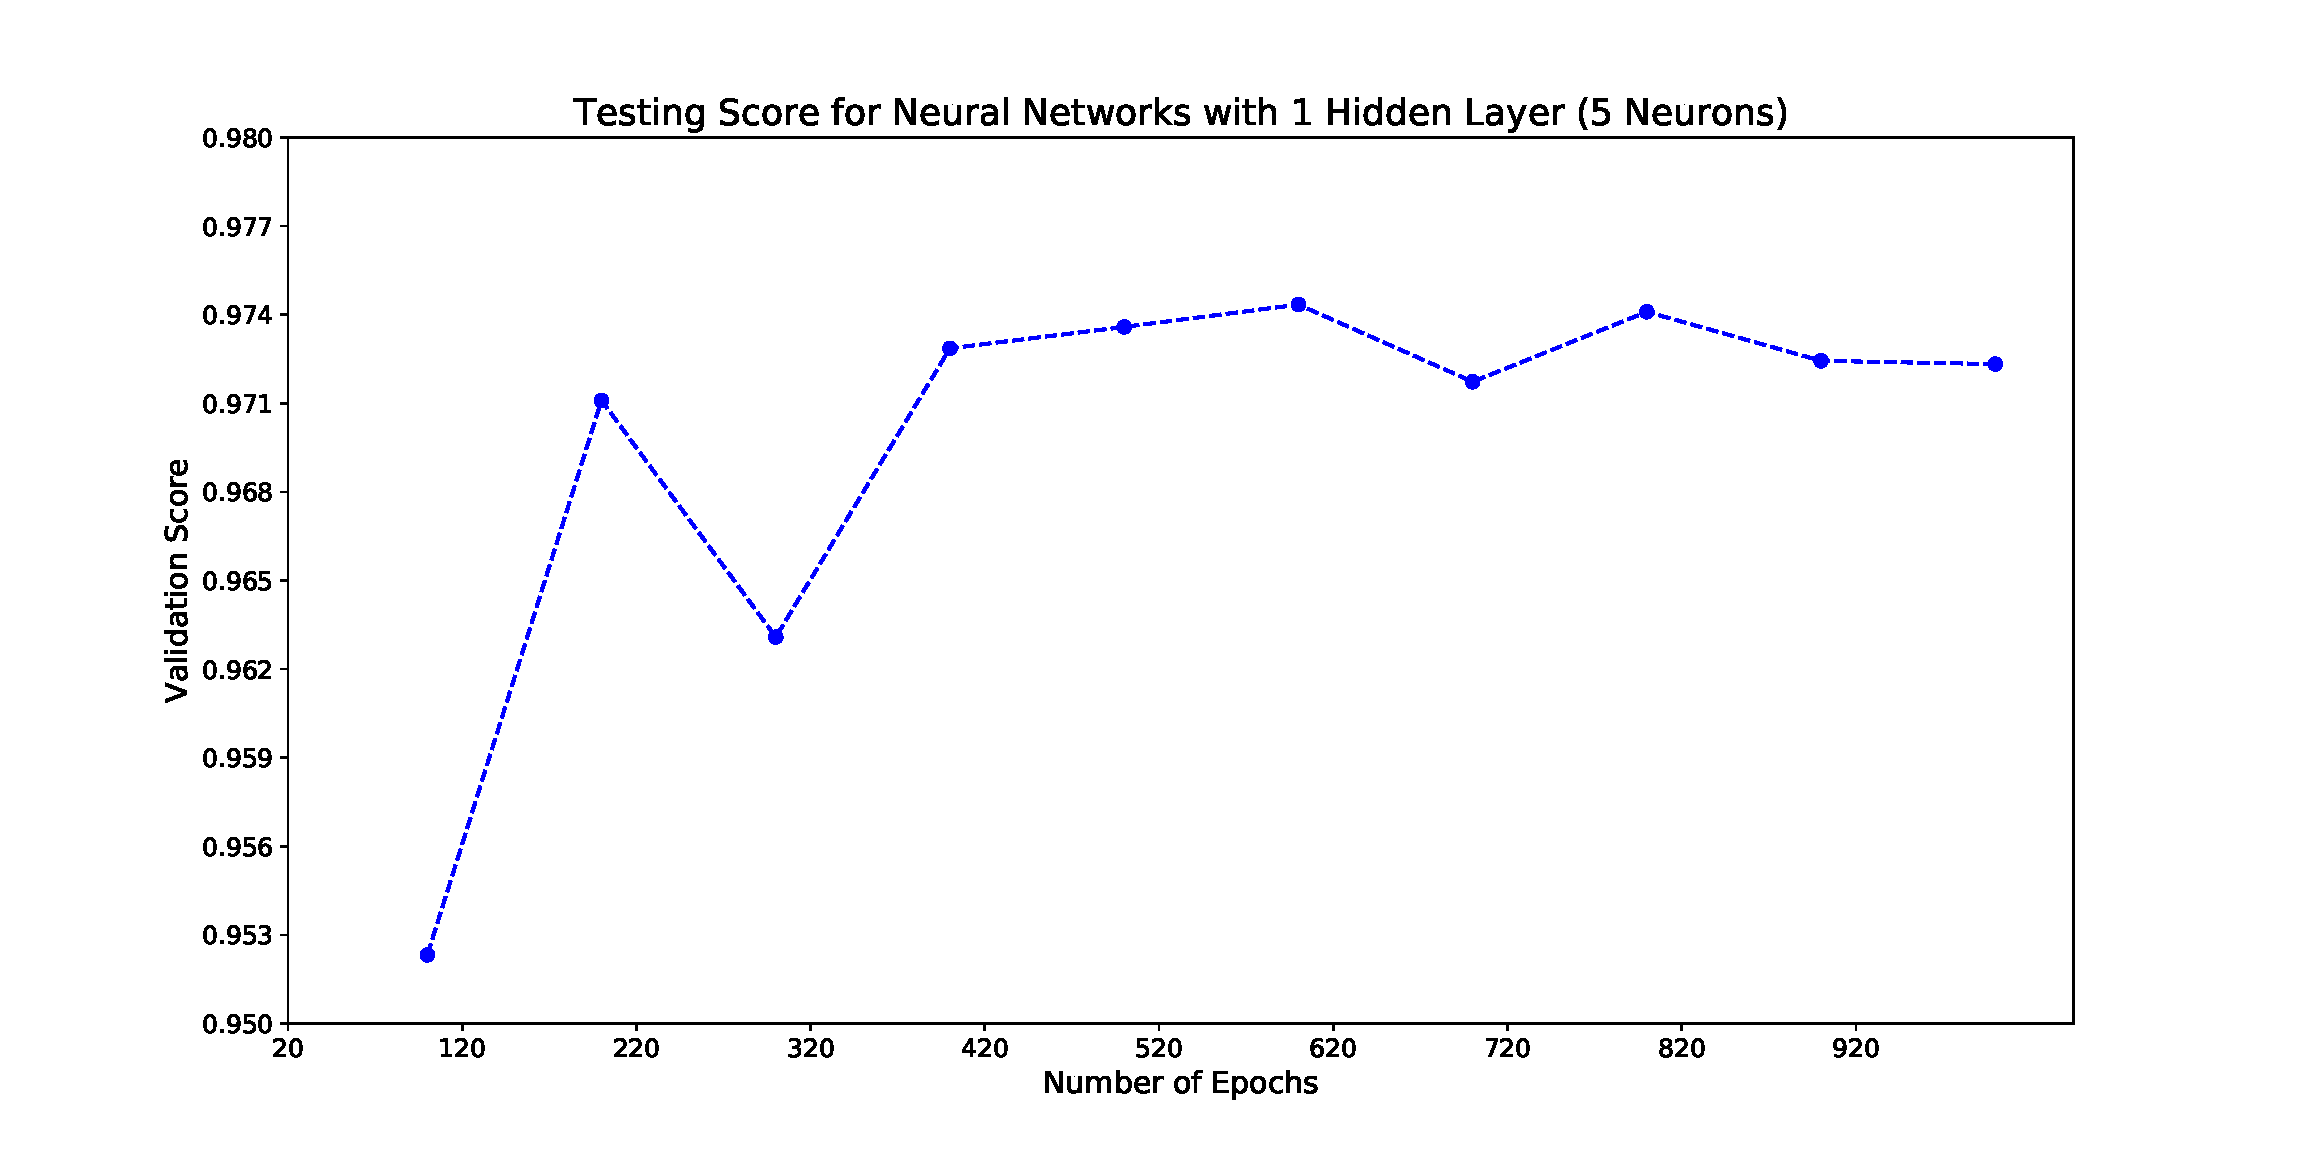
\includegraphics[width=\twopicsp\textwidth]{plots/epochsvsscore1_10seeds.pdf}
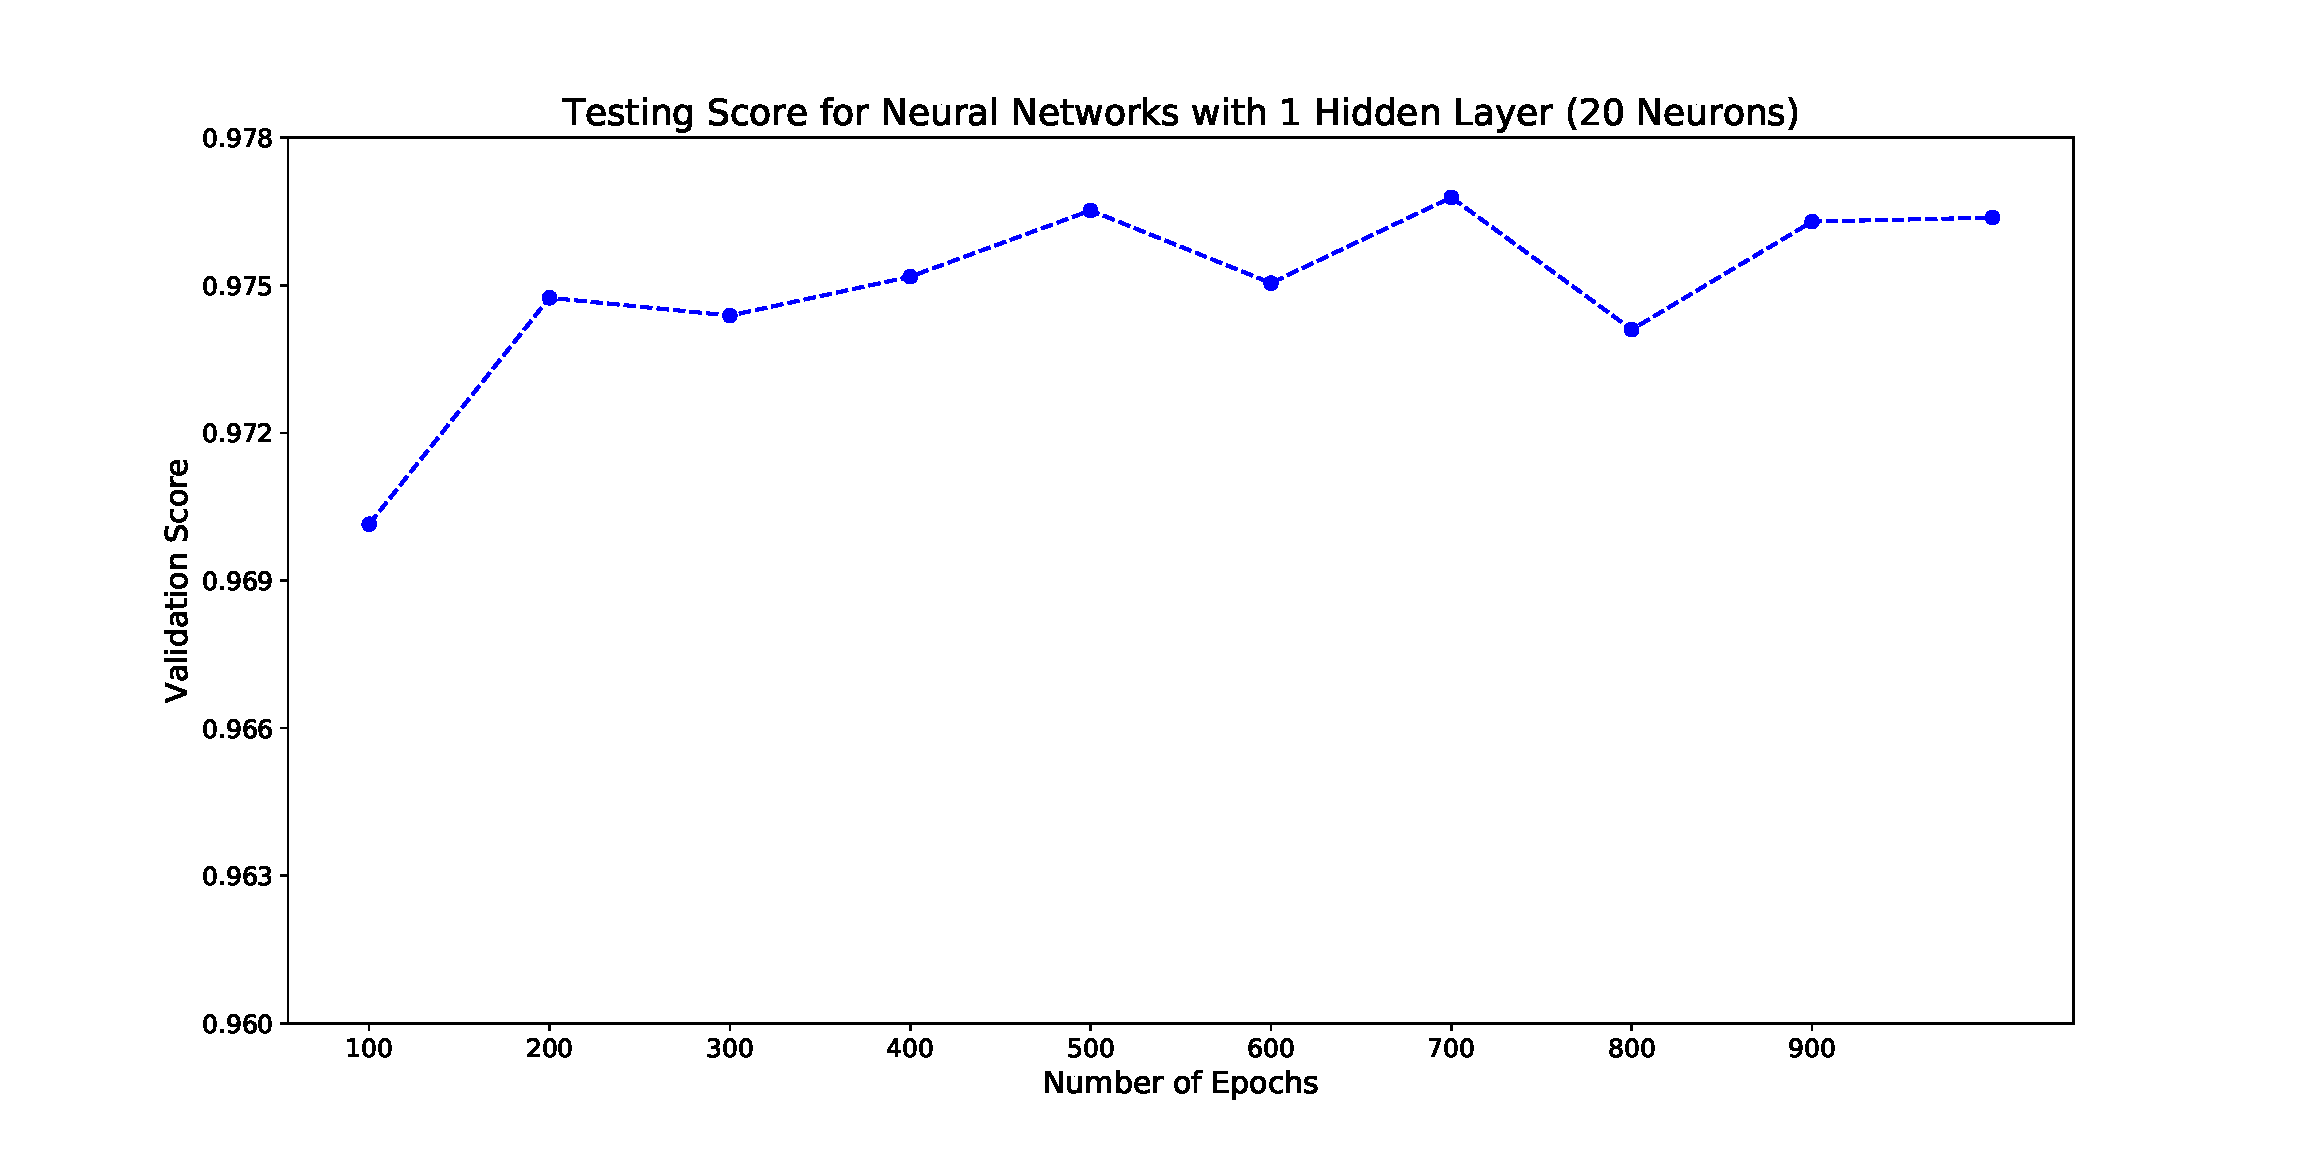
\includegraphics[width=\twopicsp\textwidth]{plots/epochsvsscore2_10seeds.pdf}
\caption{
Neural networks
}
\label{fig:Maps_data}
\end{figure*}

\begin{figure}[h]
%\centering
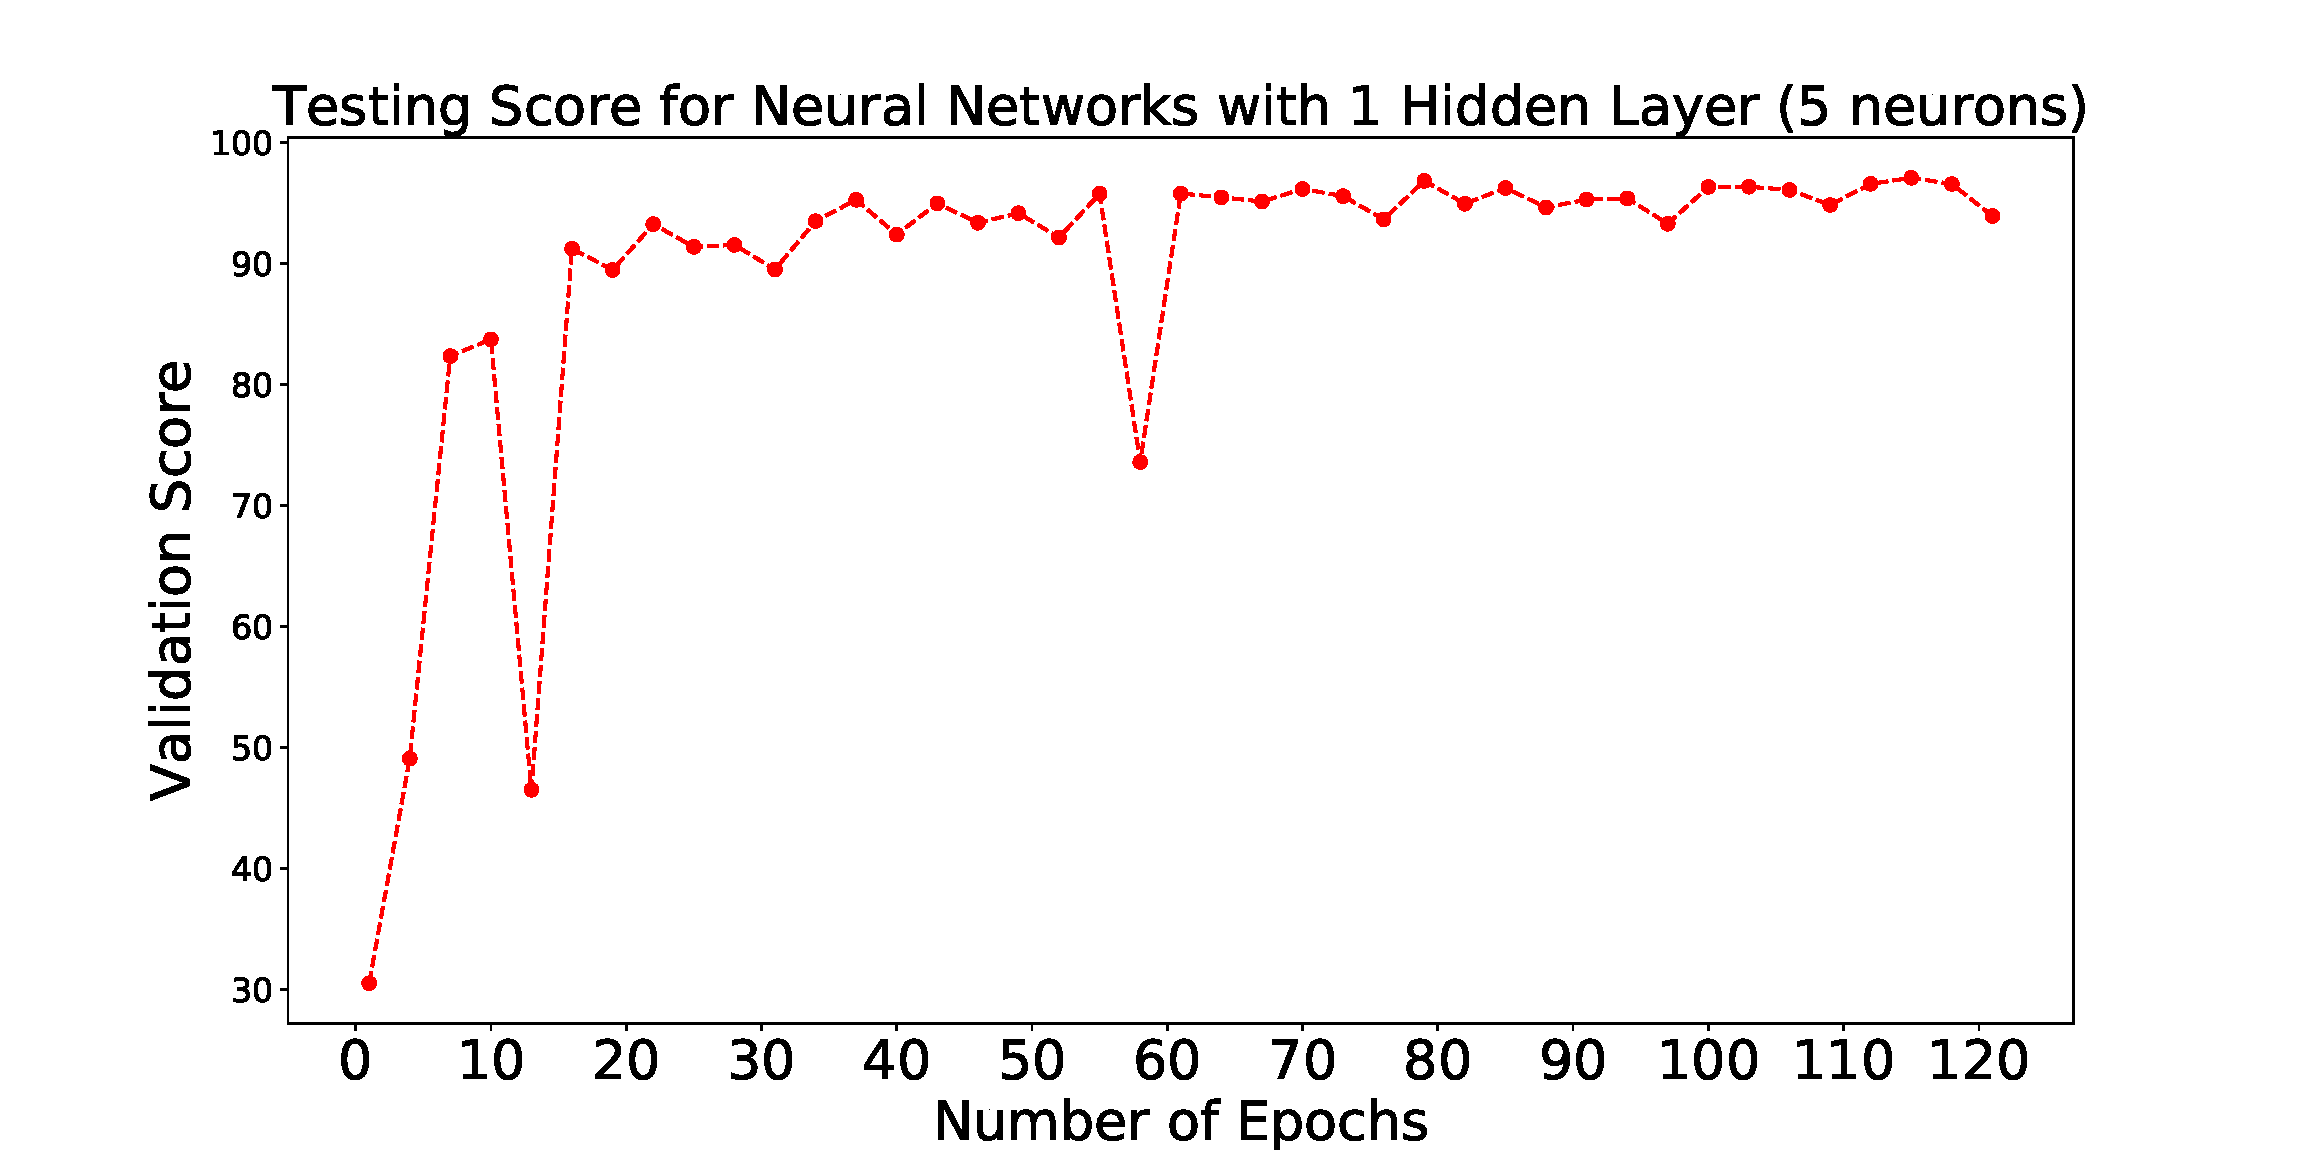
\includegraphics[width=\onepic\textwidth]{plots/epochsvsscore1_10seeds_1layer_5.pdf}
\caption{
Neural Network
}
\label{fig:Maps_data}
\end{figure}	



